% !TeX spellcheck = es_MX-SpanishMexico
%----------------------------------------------------------------------------------------------------
%                           		  ENTRE LÍNEAS DE TIERRA

% Curso: Arqueología Bíblica
% Módulo 1: Introducción, Definiciones y Conceptos
% Elabora: Rodrigo Gerardo Trejo Arriaga

%----------------------------------------------------------------------------------------------------

% FORMATO DEL DOCUMENTO


\documentclass[11pt]{article} % Letra estandar

\usepackage[utf8]{inputenc}

%\usepackage{tgadventor}
%\renewcommand{\familydefault}{\sfdefault}

\usepackage[light,math]{iwona}

\usepackage[T1]{fontenc}


\usepackage[spanish]{babel}
\addto\captionsspanish{\renewcommand{\abstractname}{\large{Introducción}}}

\usepackage[margin=1in,letterpaper]{geometry}

\usepackage{fancyhdr} % Paquete para personalizar encabezado y pie de página
\pagestyle{fancy} % Establece que personalizaremos el pie de pagina y el encabezado
\setlength{\headheight}{13.59999pt} % Establece la altura del encabezado
\fancyhead[R]{\textcolor{darkBlue}{Teoría de la Computación}} % Encabezado derecho
\fancyhead[L]{\textit{\textcolor{darkBlue}{Escuela Superior de Cómputo}}} % Encabezado izquierdo
\fancyfoot[L]{\textit{\textcolor{darkBlue}{Práctica 8}}} % Pie de página izquierdo 
\fancyfoot[R]{\textcolor{darkBlue}{\thepage}} % Pie de página  derecho
\fancyfoot[C]{} % Elimina la nueración central de páginas en el pie de página
\renewcommand{\headrulewidth}{0.5pt} % Grosor de la linea de encabezado
\renewcommand{\footrulewidth}{0.5pt} % Grosor de la linea de pie de página

\usepackage{enumitem}

\usepackage{changepage}

\usepackage{graphicx}

\usepackage{tabularx}

\setlength{\parskip}{8pt}

\usepackage{xcolor}
\definecolor{darkBlue}{rgb}{0,0,0.31}
%\definecolor{darkBlue}{rgb}{0,0,0.5}
\definecolor{munsell}{rgb}{0.0, 0.5, 0.69}
\definecolor{indigo}{rgb}{0.0, 0.25, 0.42}
\renewcommand{\footrulewidth}{2pt}
\renewcommand{\footrule}{\hbox to\headwidth{\color{darkBlue}\leaders\hrule height \footrulewidth\hfill}}

\usepackage{colortbl}

\usepackage{titlesec}
\titleformat{\section}
{\normalfont\Large\bfseries\color{darkBlue}}{\thesection.}{1em}{}

\usepackage{tabularx}

\usepackage{textcomp}

\usepackage{titling}

\usepackage{apacite}

\usepackage{amsmath}
\bibliographystyle{apacite}

%\usepackage{natbib}
%\setlength{\bibsep}{6pt}

\usepackage{setspace}

\usepackage{listings}


% Define tus propios colores en tonos de azul
\definecolor{codeblue}{rgb}{0.25,0.5,0.5}
\definecolor{backcolour}{rgb}{0.95,0.95,0.92}
\definecolor{commentblue}{rgb}{0.3,0.3,0.6}
\definecolor{keywordblue}{rgb}{0.2,0.2,0.7}
\definecolor{stringblue}{rgb}{0.15,0.2,0.9}

\lstdefinestyle{bluepythonstyle}{
	language=Python,
	basicstyle=\ttfamily\small,
	commentstyle=\color{commentblue},
	keywordstyle=\color{keywordblue},
	numberstyle=\tiny\color{codeblue},
	stringstyle=\color{stringblue},
	backgroundcolor=\color{backcolour},
	breaklines=true,
	captionpos=b,
	abovecaptionskip=1\baselineskip,
	showstringspaces=false,
	frame=lines,
	numbers=left,
	xleftmargin=\parindent,
	tabsize=4
}
\lstset{style=bluepythonstyle}



\renewcommand{\thesection}{\Roman{section}}

%----------------------------------------------------------------------------------------------------
% CUERPO DEL DOCUMENTO

\begin{document}
	
	\begin{titlepage}
		\centering
		{
\includegraphics[width=0.25\textwidth]{descarga}\par}
		\vspace{0.5cm}
		{\bfseries\huge Escuela Superior de Cómputo \par}
		\vspace{0.7cm}
		{\scshape\LARGE Teoría de la Computación \par}
		\vspace{0.3cm}
		\vspace{3.1cm}
		{\scshape \Huge \textbf{Práctica 8:}  \par}
		\vspace{0.03cm}
		{{\LARGE \textit{LENGUAJES LIBRES DE CONTEXTO\\ \vspace{3mm} BAKUS-NAUR CONDITIONAL IF}} \par}
		%\vfill
		\vspace{3.5cm}
		{\Large Autor: \par}
		{\Large Rodrigo Gerardo Trejo Arriaga \par}
		%\vfill
		\vspace{3cm}
		{\Large Diciembre 2023 \par}
	\end{titlepage}
	
	\begin{center}
		\vspace*{0.1cm}
		{\huge \textcolor{darkBlue}{\textbf{Práctica 8:}} \par}
		
		{\Large \textcolor{darkBlue}{\textbf{\textit{LENGUAJES LIBRES DE CONTEXTO\\ \vspace{3mm} BAKUS-NAUR CONDITIONAL IF}}}}
	\end{center}
	
	
	\section{Introducción}
	Los \textbf{lenguajes libres de contexto} (CFL) son un tipo de lenguaje formal que son generados por \textbf{gramáticas libres de contexto} (CFG). Son esenciales en el diseño de lenguajes de programación y en la teoría de compiladores. Estos lenguajes tienen la capacidad de describir la sintaxis de lenguajes de programación y estructuras anidadas, lo que los hace más expresivos que los lenguajes regulares [1].
	
	\section{Gramáticas Libres de Contexto}
	Una gramática libre de contexto se define como una cuádrupla \( G = (V, \Sigma, R, S) \) donde [1]:
	\begin{itemize}
		\item \( V \) es un conjunto finito de \textit{variables} sintácticas.
		\item \( \Sigma \) es un conjunto finito de \textit{símbolos terminales} que constituyen el alfabeto del lenguaje.
		\item \( R \) es un conjunto finito de \textit{reglas de producción} de la forma \( A \rightarrow \beta \), donde \( A \in V \) y \( \beta \in (V \cup \Sigma)^* \).
		\item \( S \in V \) es el \textit{símbolo de inicio}.
	\end{itemize}
	
	\section{Notación de Backus-Naur (BNF)}
	La \textbf{Notación de Backus-Naur} es una metasintaxis, es decir, una notación para describir otras notaciones. Se utiliza para expresar las reglas gramaticales de lenguajes de programación y datos[2].
	
	Una gramática en BNF tiene la siguiente forma:
	\begin{verbatim}
		<símbolo> ::= _expresión_
	\end{verbatim}
	donde \( <símbolo> \) es una variable no terminal y la \_expresión\_ puede ser una combinación de terminales y/o no terminales[2].
	
	
	\section{Elementos Opcionales en BNF}
	Los elementos opcionales en BNF se indican con corchetes \([ \ldots ]\). Esto significa que el contenido dentro de los corchetes puede estar presente o no en la cadena derivada del no terminal.
	
	Considere la siguiente regla de producción:
	\begin{verbatim}
		<statement> ::= if <condition> then <statement> [else <statement>]
	\end{verbatim}
	Aquí, la presencia de \textit{else <statement>} es opcional. Esto significa que un \textit{<statement>} puede ser simplemente una estructura 'if-then', o puede ser extendida a 'if-then-else'.
	
	\section{BNF Condicional IF}
	La estructura condicional 'if' es un elemento fundamental en muchos lenguajes de programación. En BNF, una gramática condicional 'if' se puede expresar como sigue [3]:
	
	La gramática para una estructura 'if-then-else' puede representarse en BNF de la siguiente manera:
	\begin{verbatim}
		<if-statement> ::= if <condition> then <statement> <optional-else>
		<optional-else> ::= else <statement> | \epsilon
	\end{verbatim}
	El símbolo \( \epsilon \) representa la cadena vacía, indicando que el elemento 'else' puede estar ausente.
	
	\section{Instrucciones}
	
	El objetivo de este programa es realizar derivaciones automáticas de la gramática Backus-Naur que define la estructura condicional IF. La gramática está definida como sigue:
	\begin{lstlisting}
		S -> iCtSA
		A -> ;eS | \epsilon
	\end{lstlisting}
	El programa derivará la gramática aleatoriamente hasta crear una cantidad de estructuras IF determinada por el usuario o por la propia máquina.
	
	\subsection*{Requerimientos del Programa}
	El programa deberá:
	\begin{itemize}
		\item Solicitar al usuario el número de estructuras IF que desea generar.
		\item Realizar las derivaciones de forma aleatoria, mostrando cada paso del proceso.
		\item Limitar el número máximo de derivaciones a 1000.
		\item Guardar la traza de todas las derivaciones en un archivo de texto.
		\item Generar y almacenar en otro archivo el pseudo-código resultante de la cadena generada por la gramática.
	\end{itemize}
	
	\subsection*{Pseudo-código}
	El pseudo-código que representa la cadena generada deberá reflejar la estructura lógica de las condicionales IF anidadas y las correspondientes ramas ELSE, si las hay.
	
	
	
	\section{Resultados}
	
	Se ejecuta 3 veces el modo manual con una longitud de 5, para que se observe como en cada ejecución los resultados son diferentes debido a la característica random del programa.
	
	
	\begin{figure}[h]
		\centering
		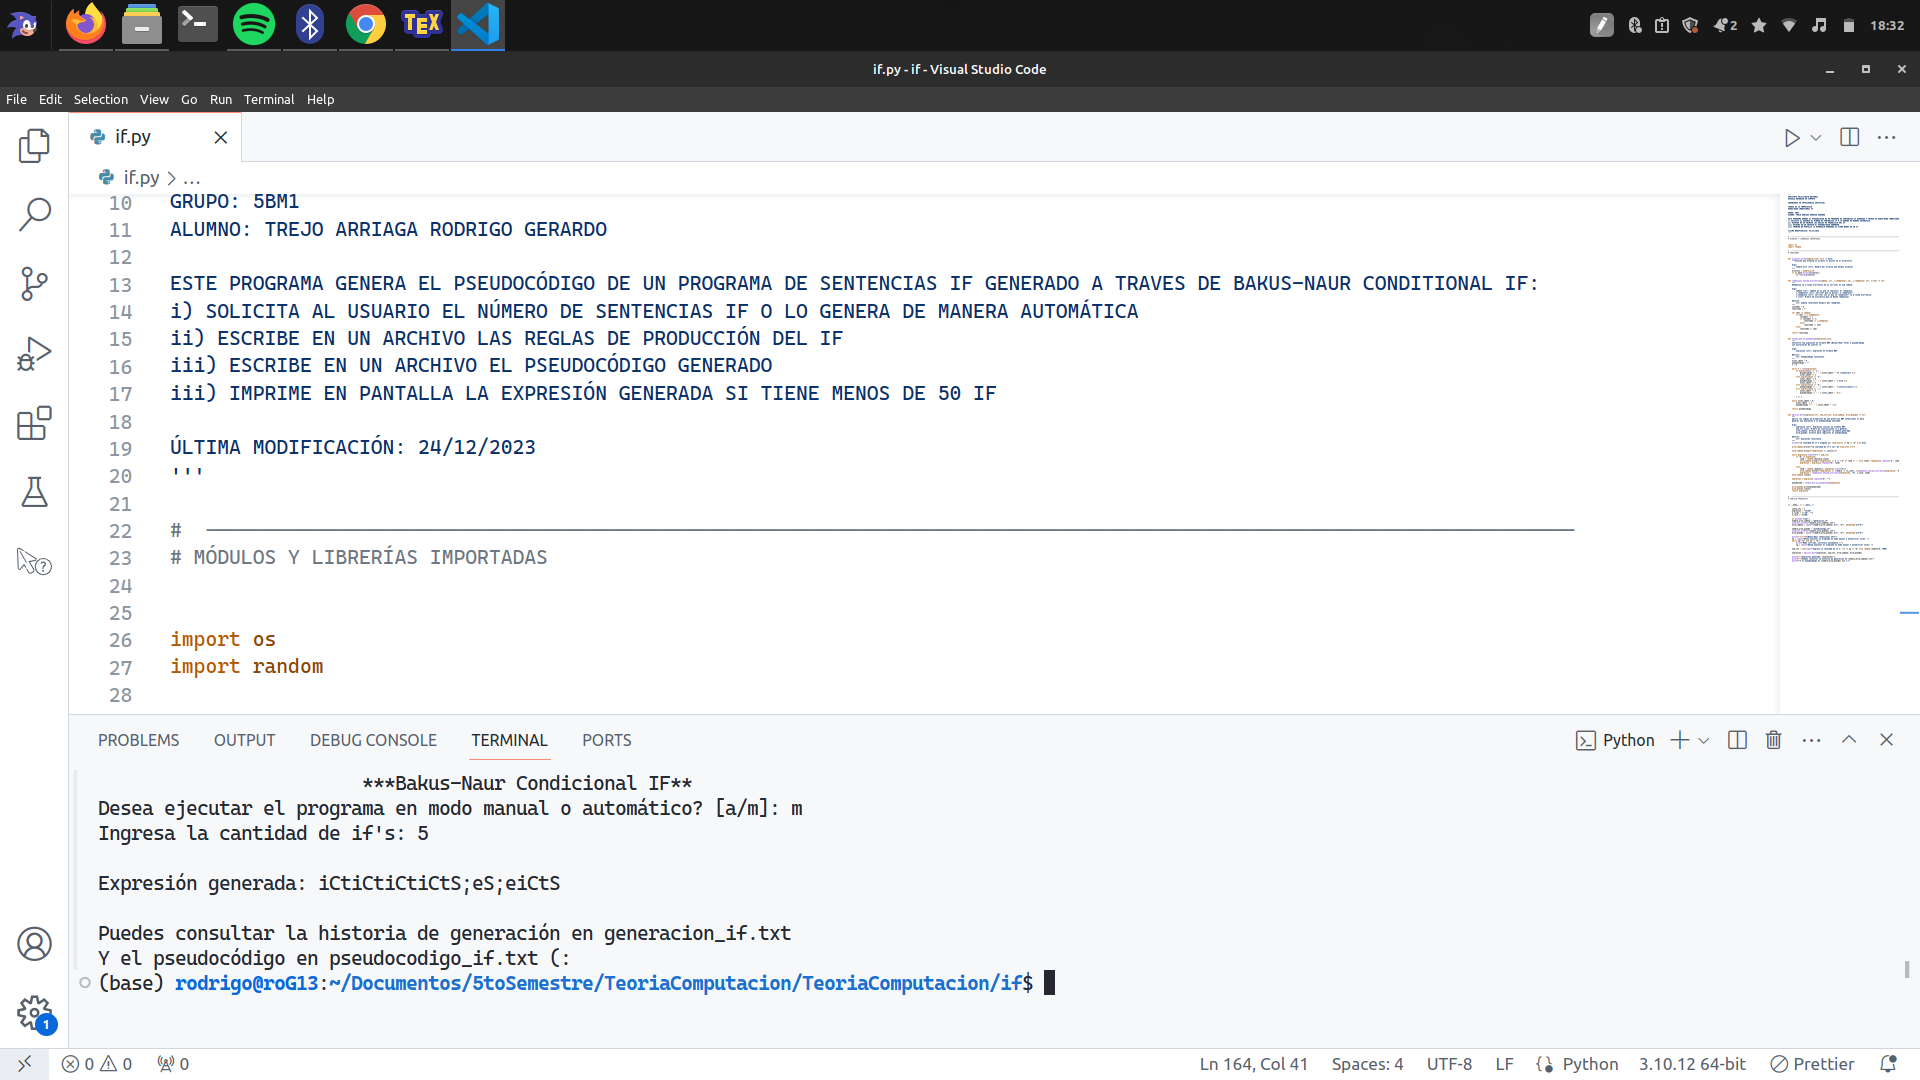
\includegraphics[width=0.8\textwidth]{manual1.png}
		\caption{Modo manual 1 - Longitud 5}
	\end{figure}
	

	
	\newpage
	
	\begin{figure}[h]
		\centering
		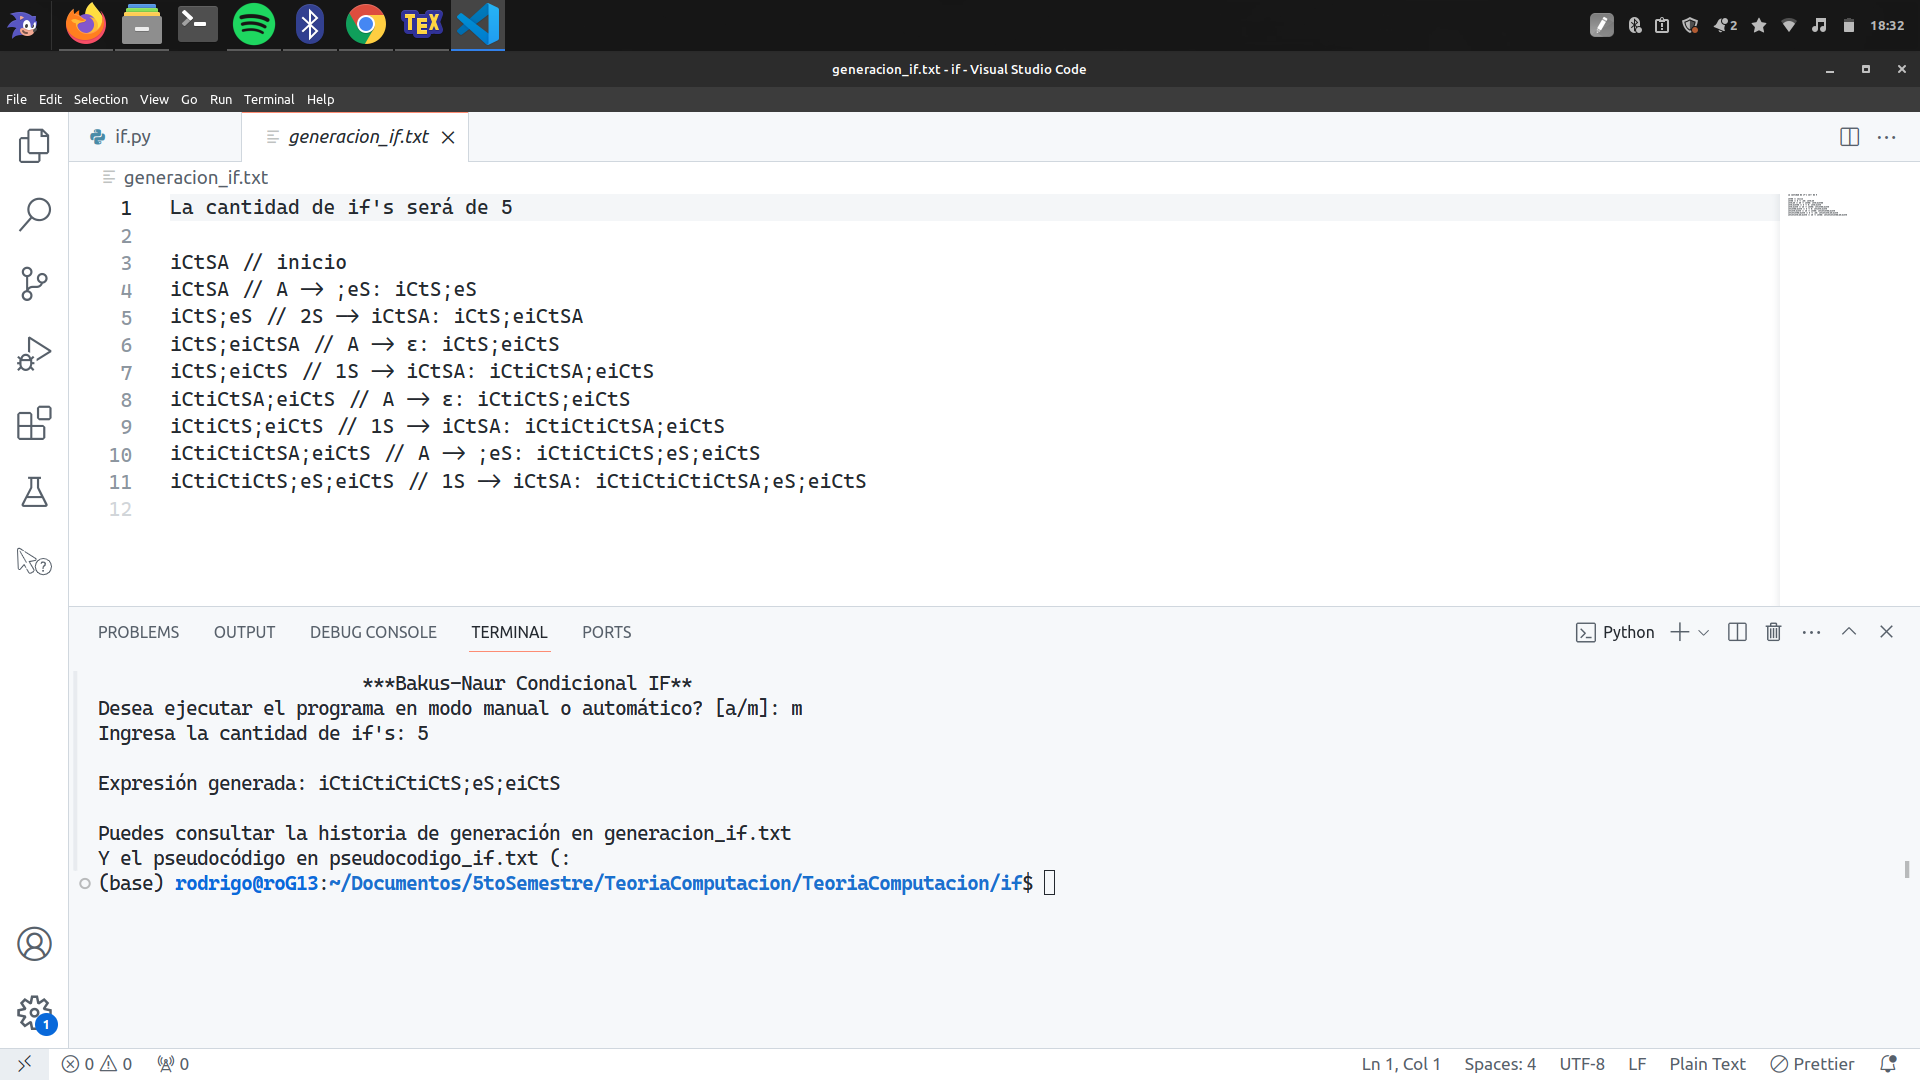
\includegraphics[width=0.8\textwidth]{arch1,1}
		\caption{Generación del Modo manual 1 - Longitud 5}
	\end{figure}
	
	\begin{figure}[h]
		\centering
		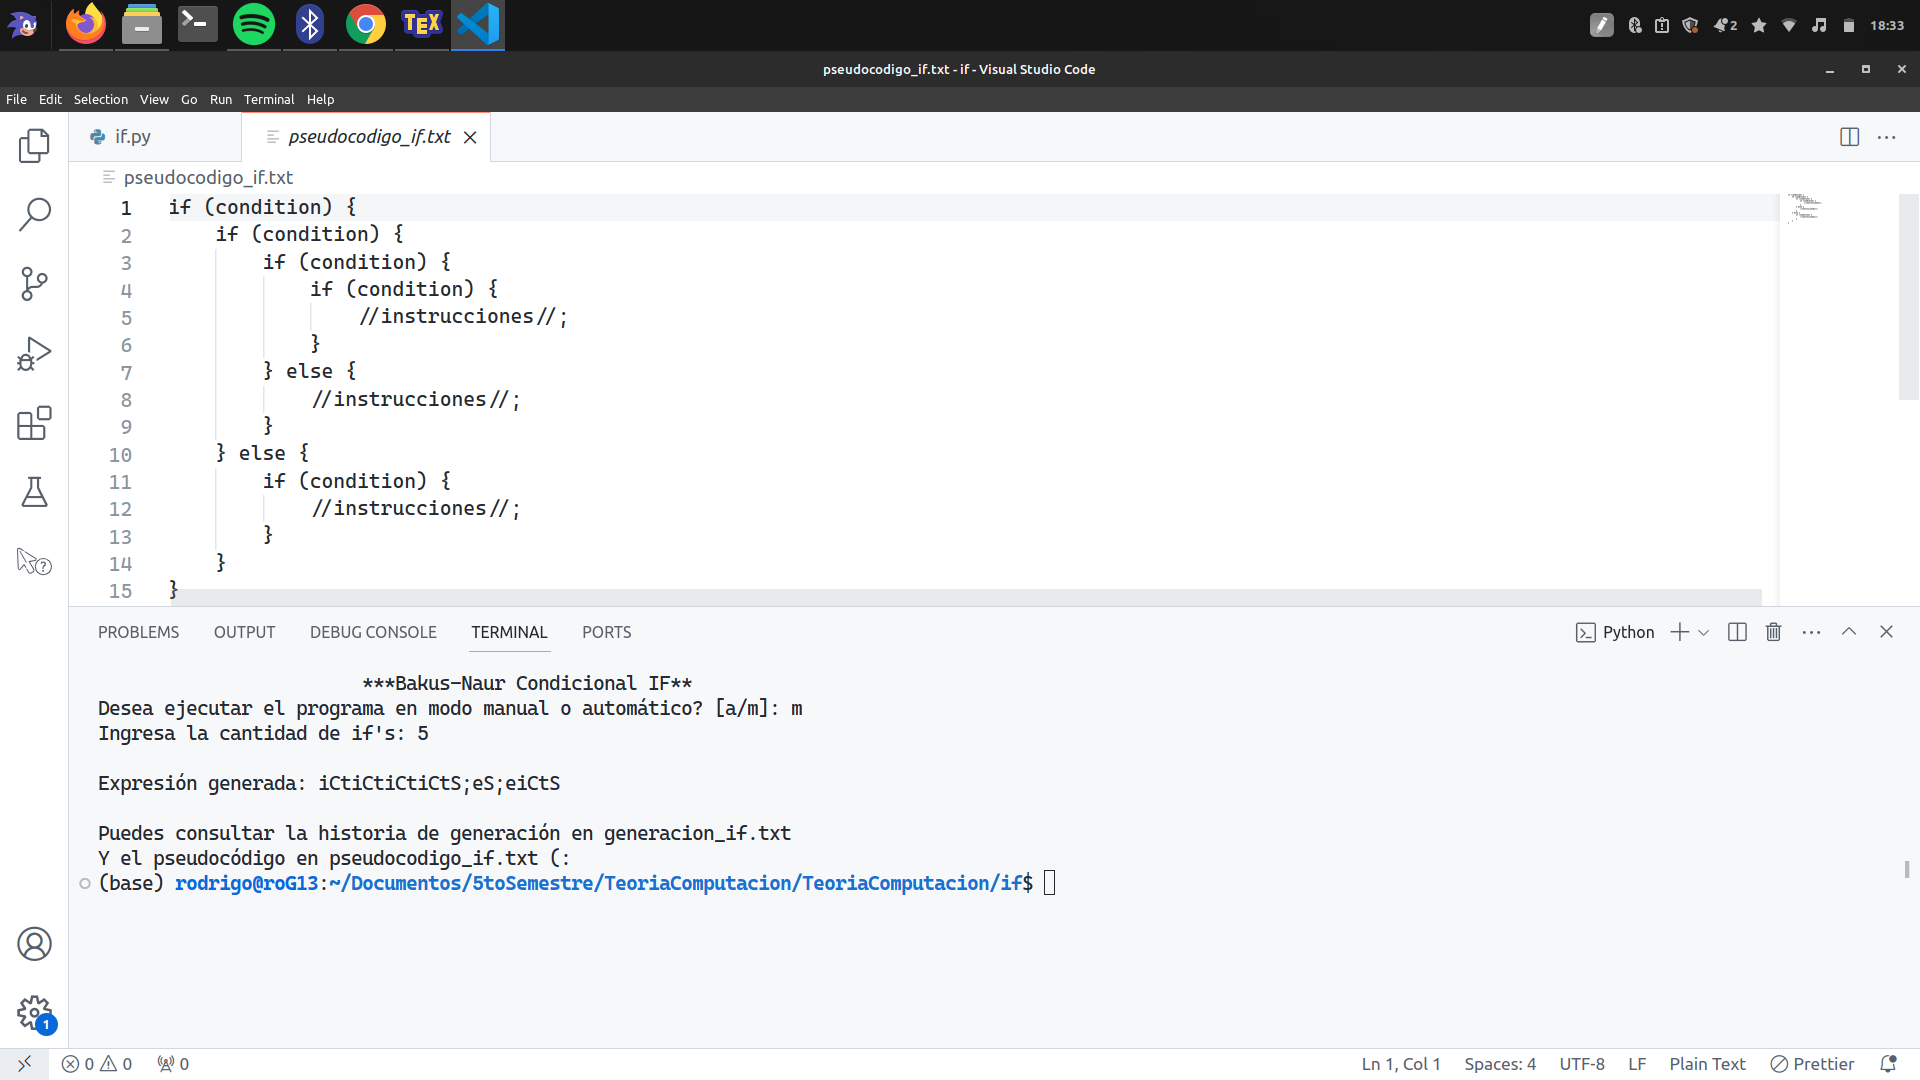
\includegraphics[width=0.8\textwidth]{manual1,2}
		\caption{Pseudocódigo del Modo manual 1 - Longitud 5}
	\end{figure}
	

	
	\newpage
	
	\begin{figure}[h]
		\centering
		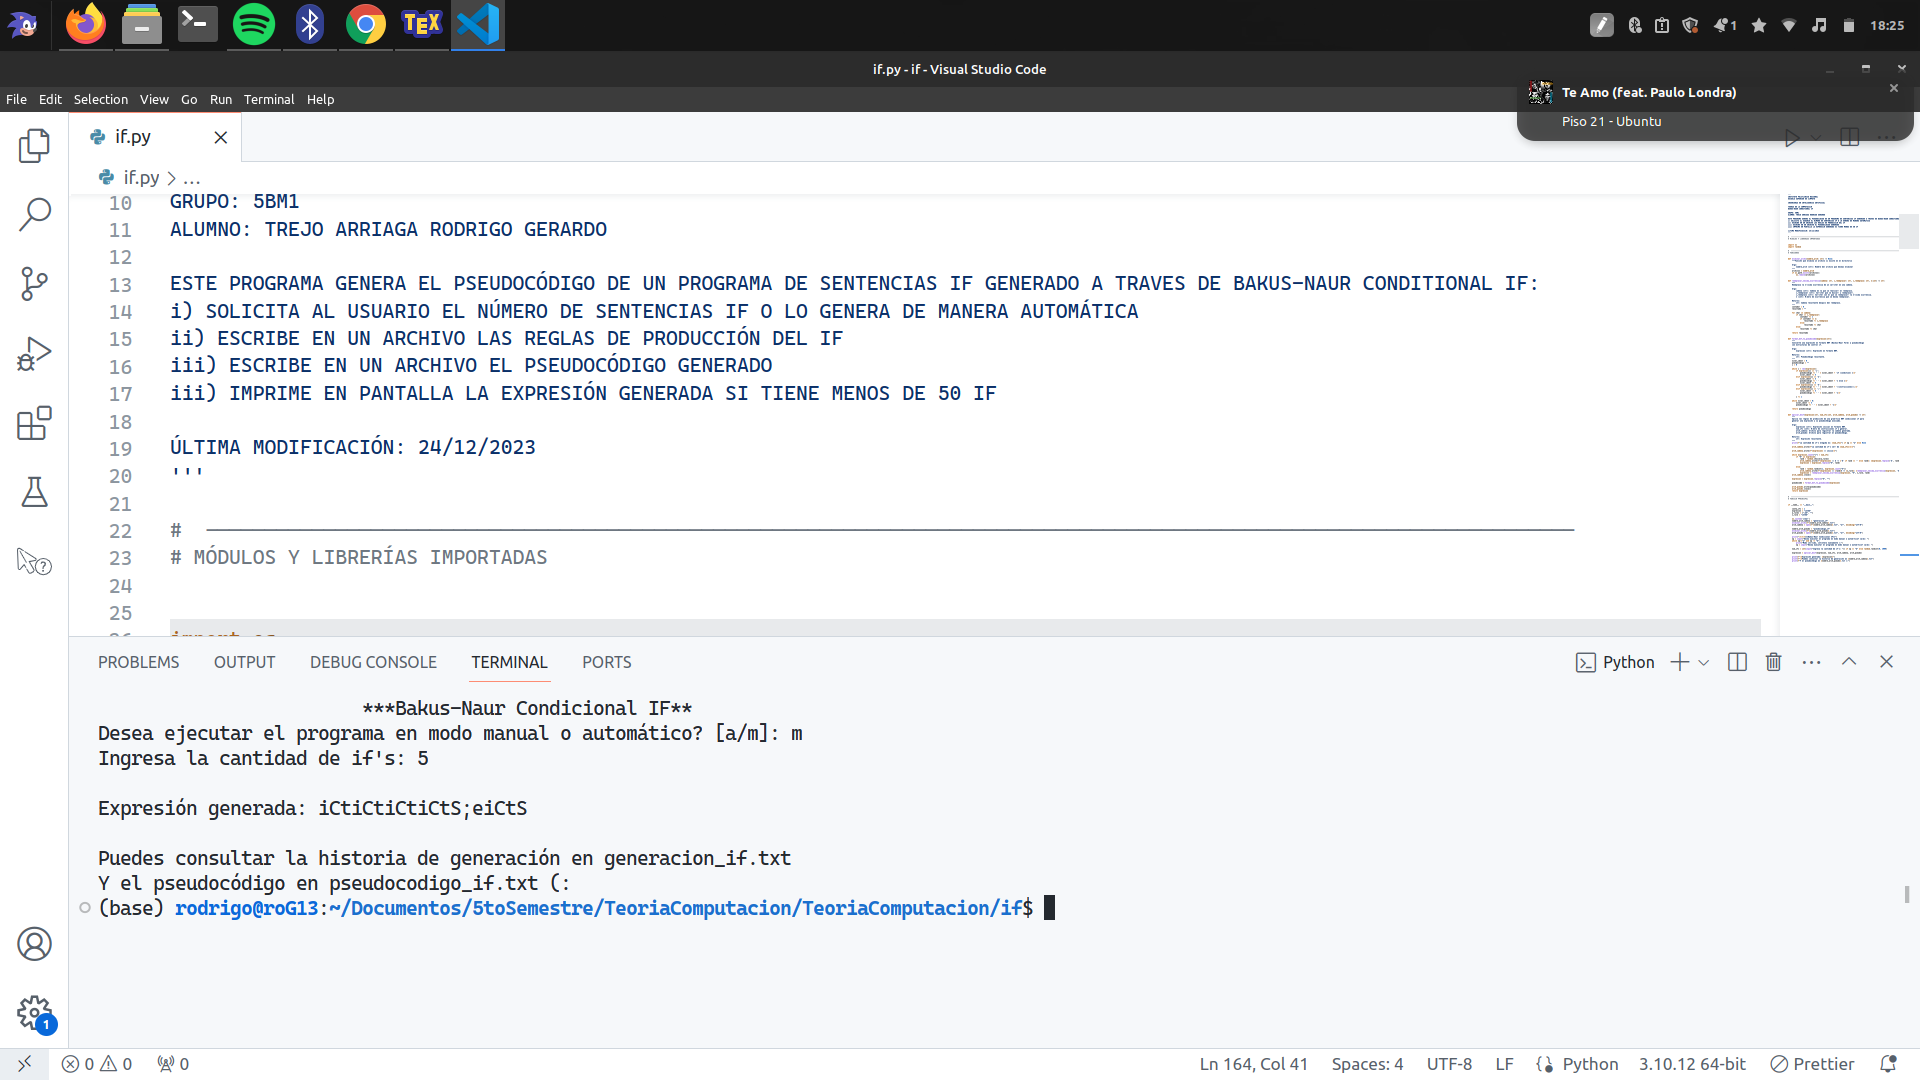
\includegraphics[width=0.8\textwidth]{manual2.png}
		\caption{Modo manual 2 - Longitud 5}
	\end{figure}
	
	\begin{figure}[h]
		\centering
		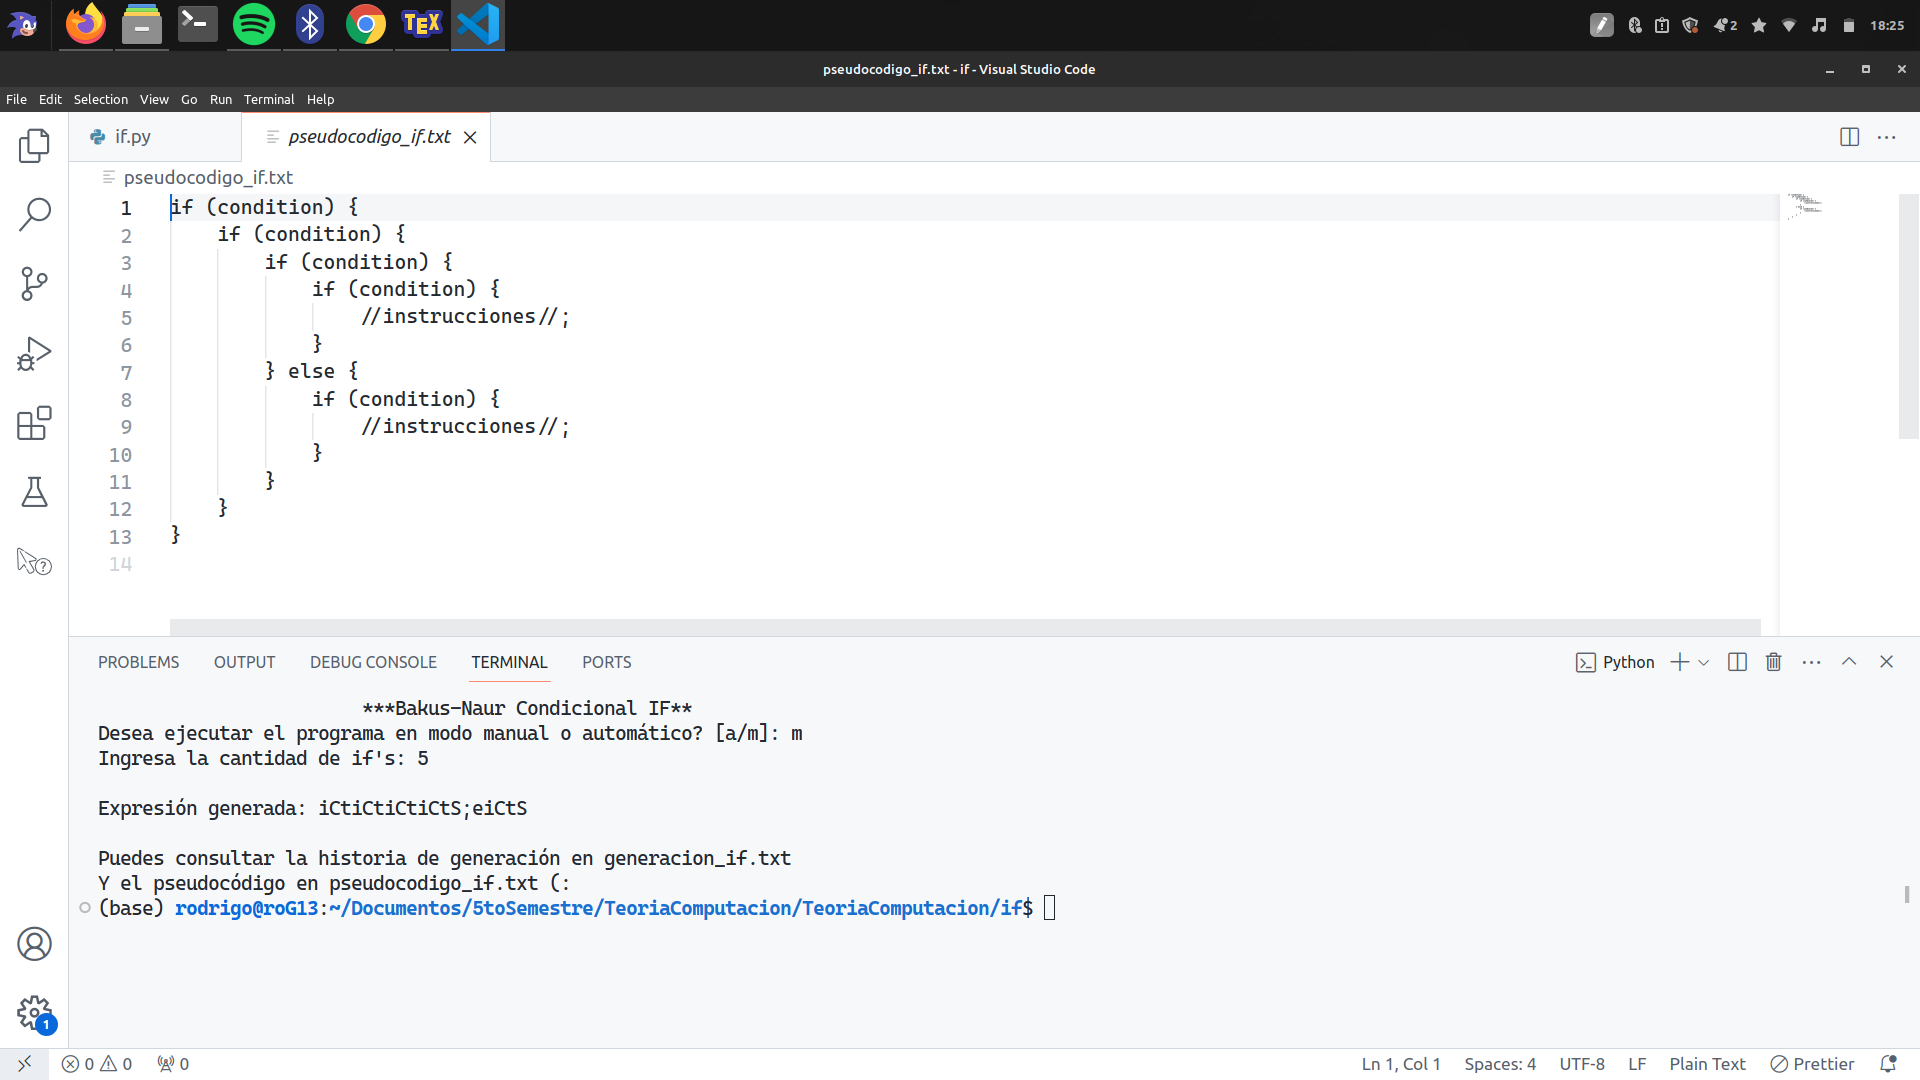
\includegraphics[width=0.8\textwidth]{arch2,1}
		\caption{Pseudocódigo del Modo manual 2 - Longitud 5}
	\end{figure}
	
	\newpage
	
	
	\begin{figure}[h]
		\centering
		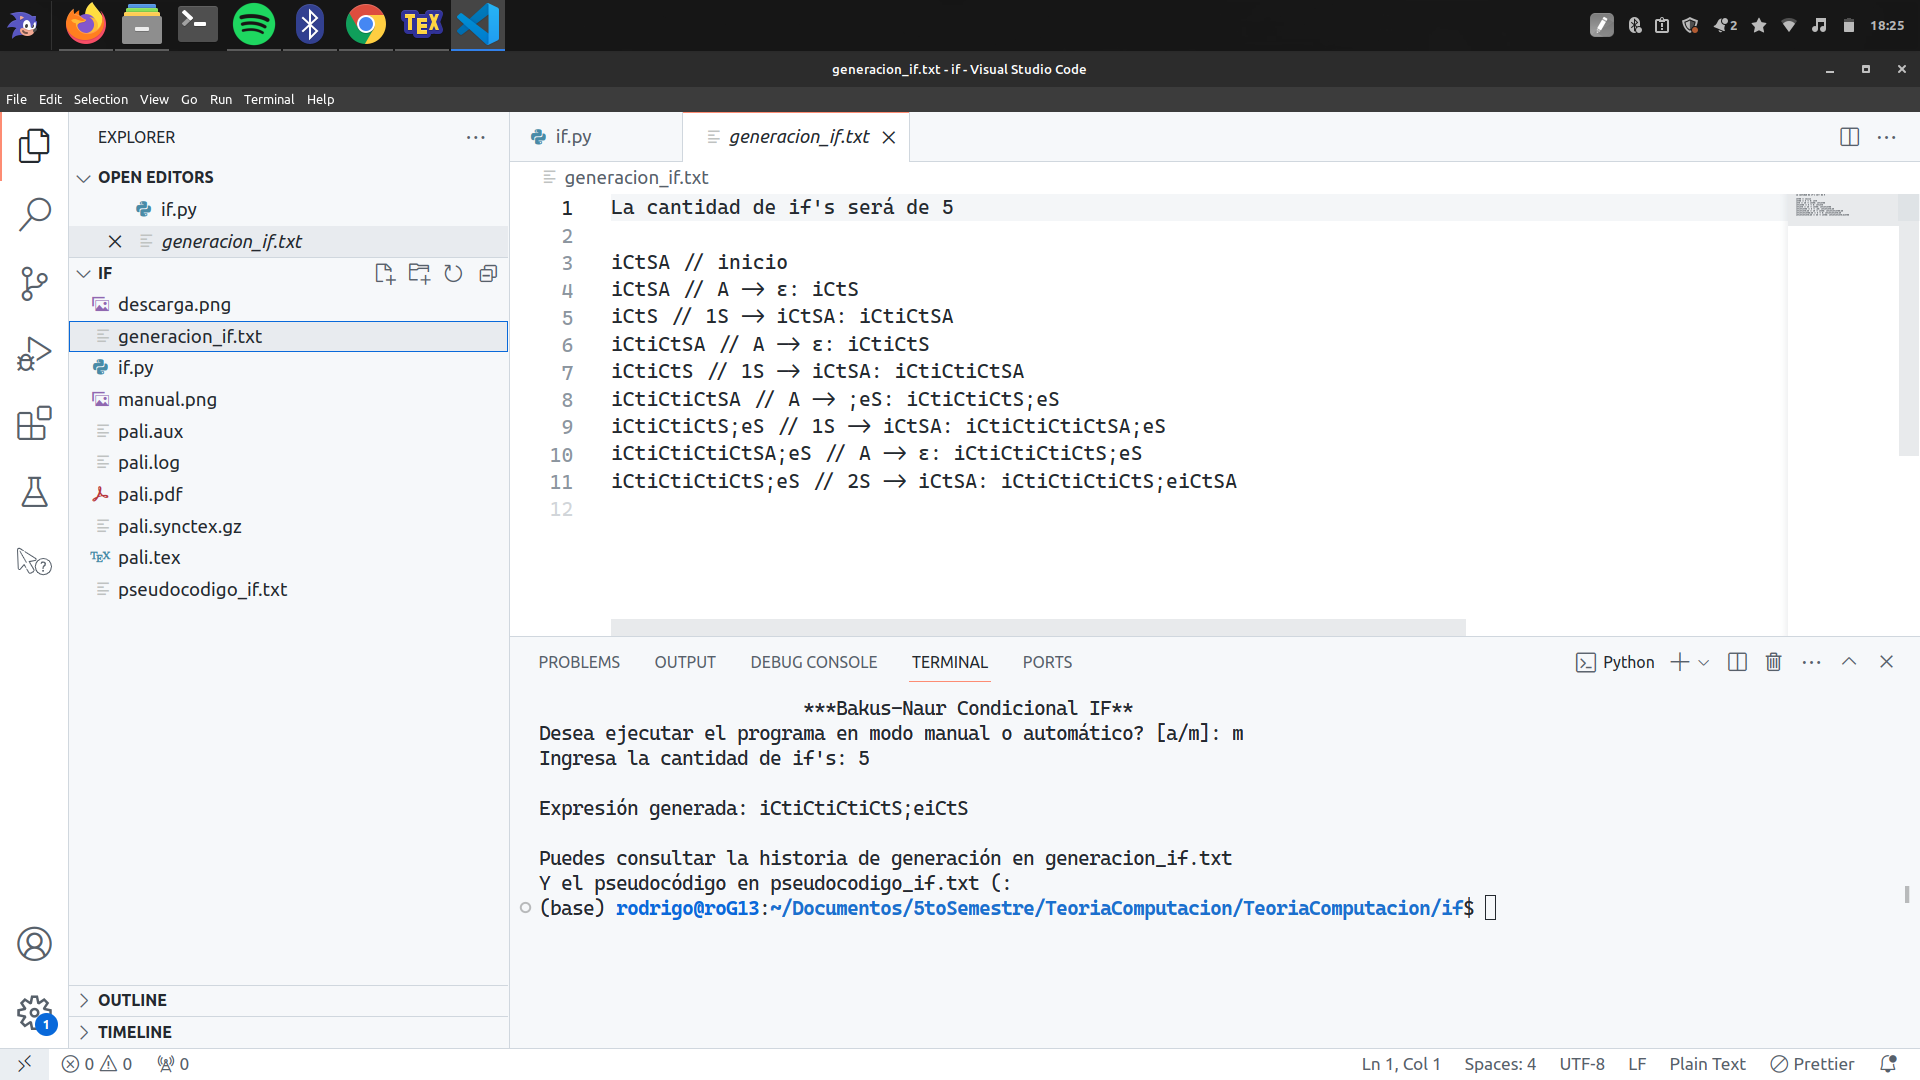
\includegraphics[width=0.8\textwidth]{arch2,2}
		\caption{Generación del Modo manual 2 - Longitud 5}
	\end{figure}
	
	\begin{figure}[h]
		\centering
		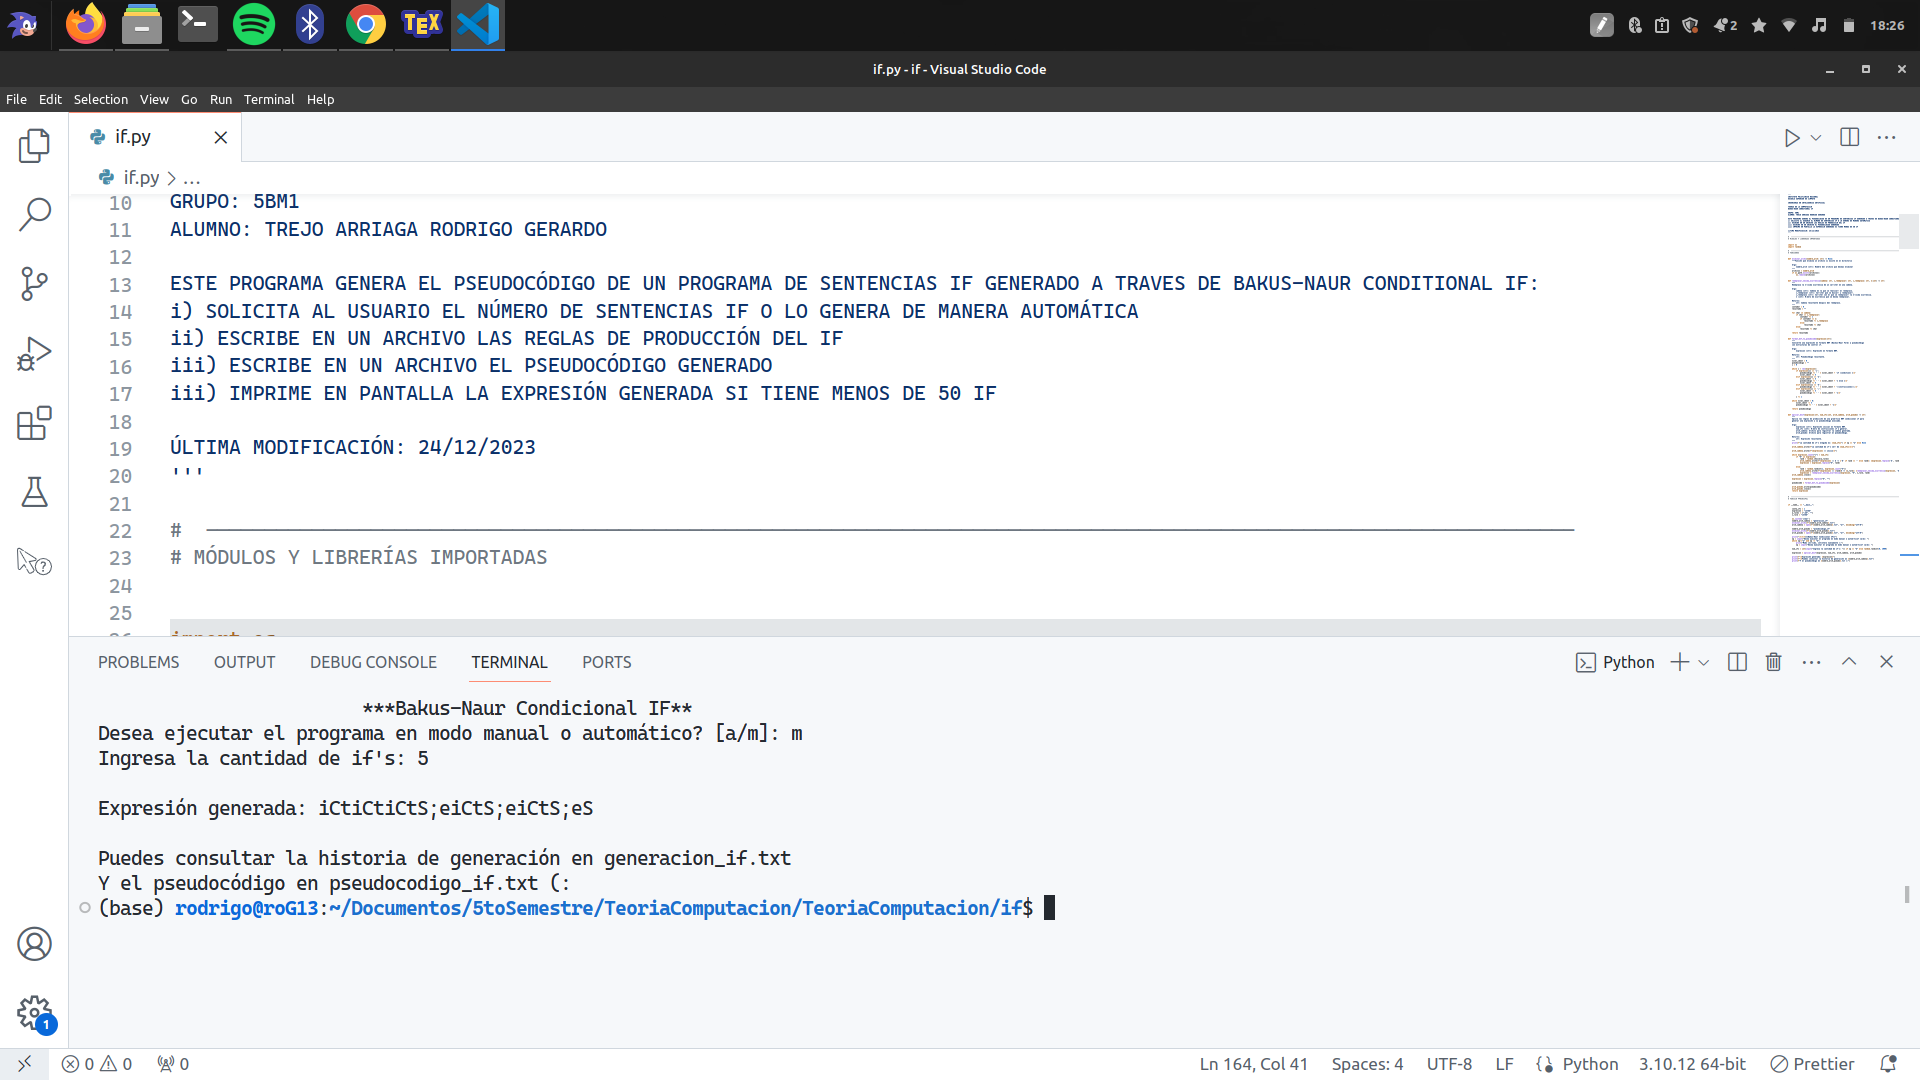
\includegraphics[width=0.8\textwidth]{manual3.png}
		\caption{Modo manual 3 - Longitud 5}
	\end{figure}
	
	\newpage
	
	\newpage
	
	\begin{figure}[h]
		\centering
		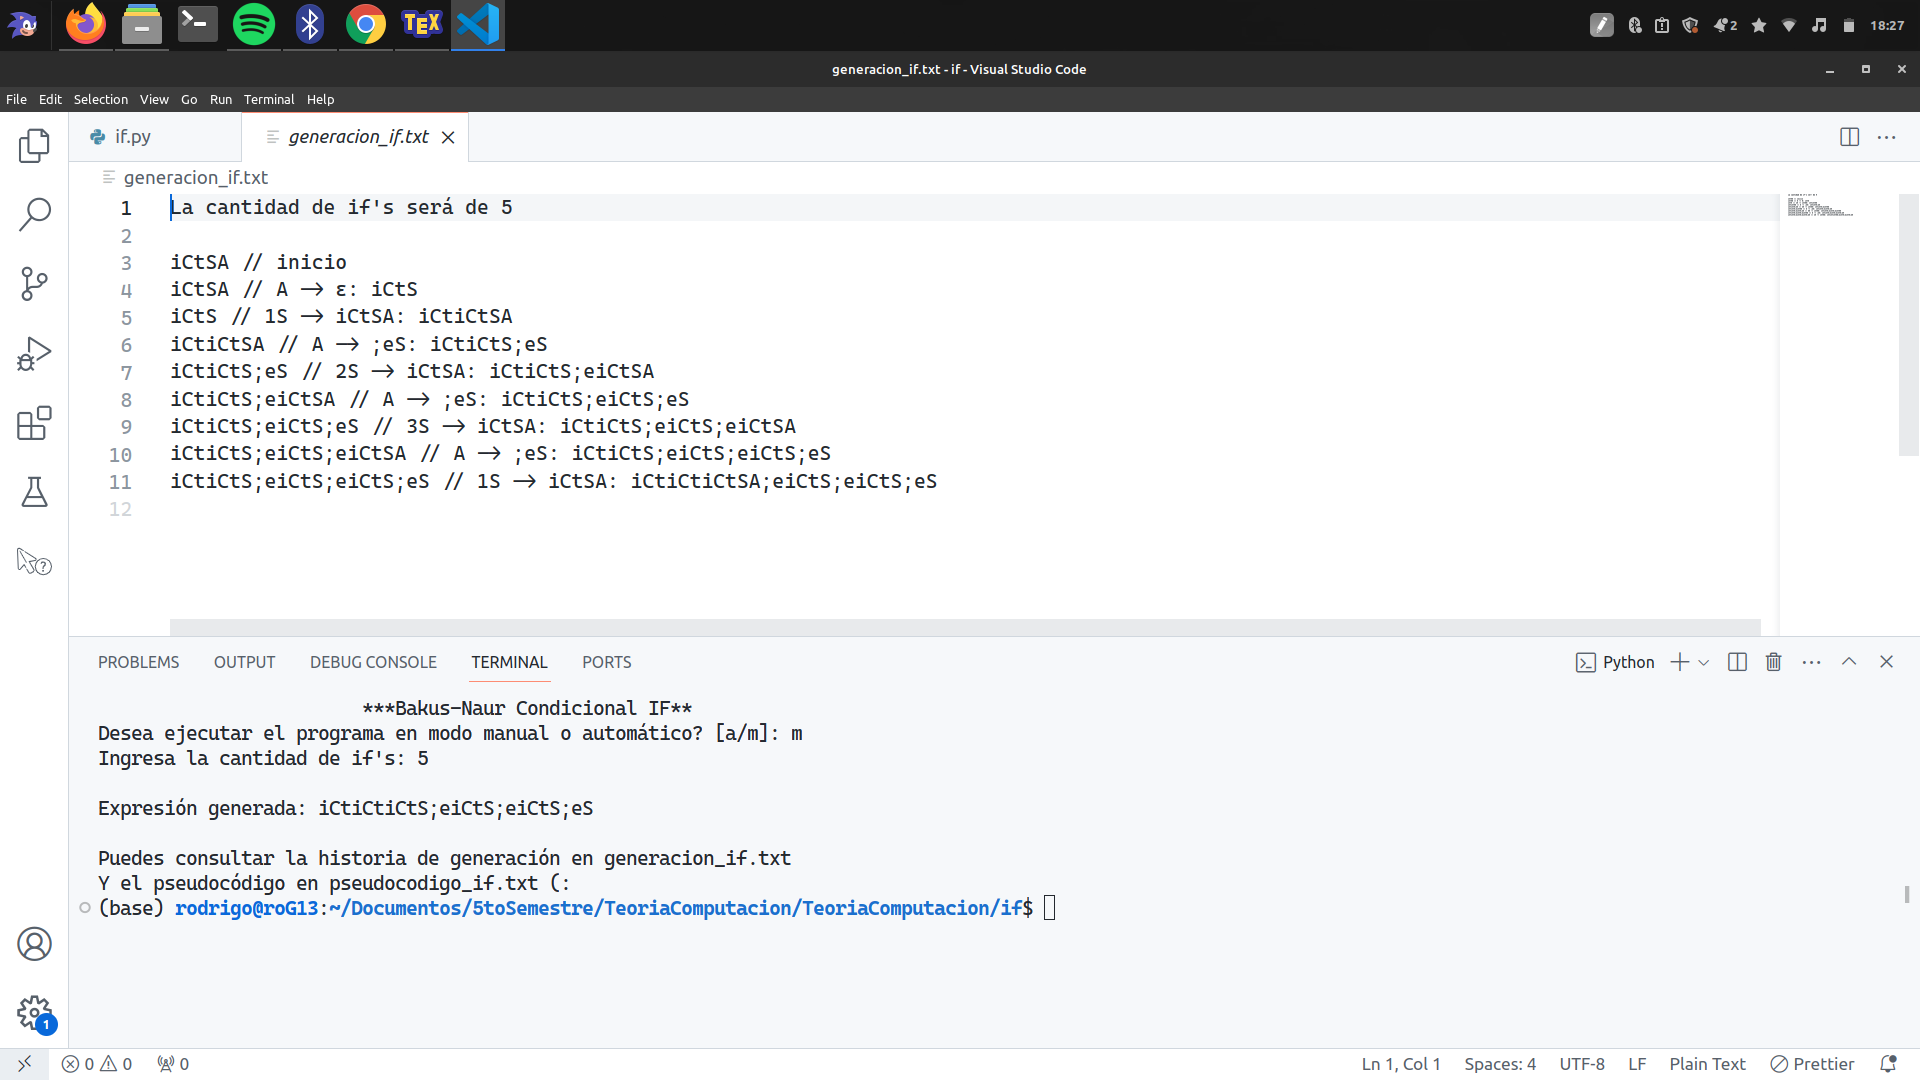
\includegraphics[width=0.8\textwidth]{arch3,1}
		\caption{Generación del Modo manual 3 - Longitud 5}
	\end{figure}
	
	\begin{figure}[h]
		\centering
		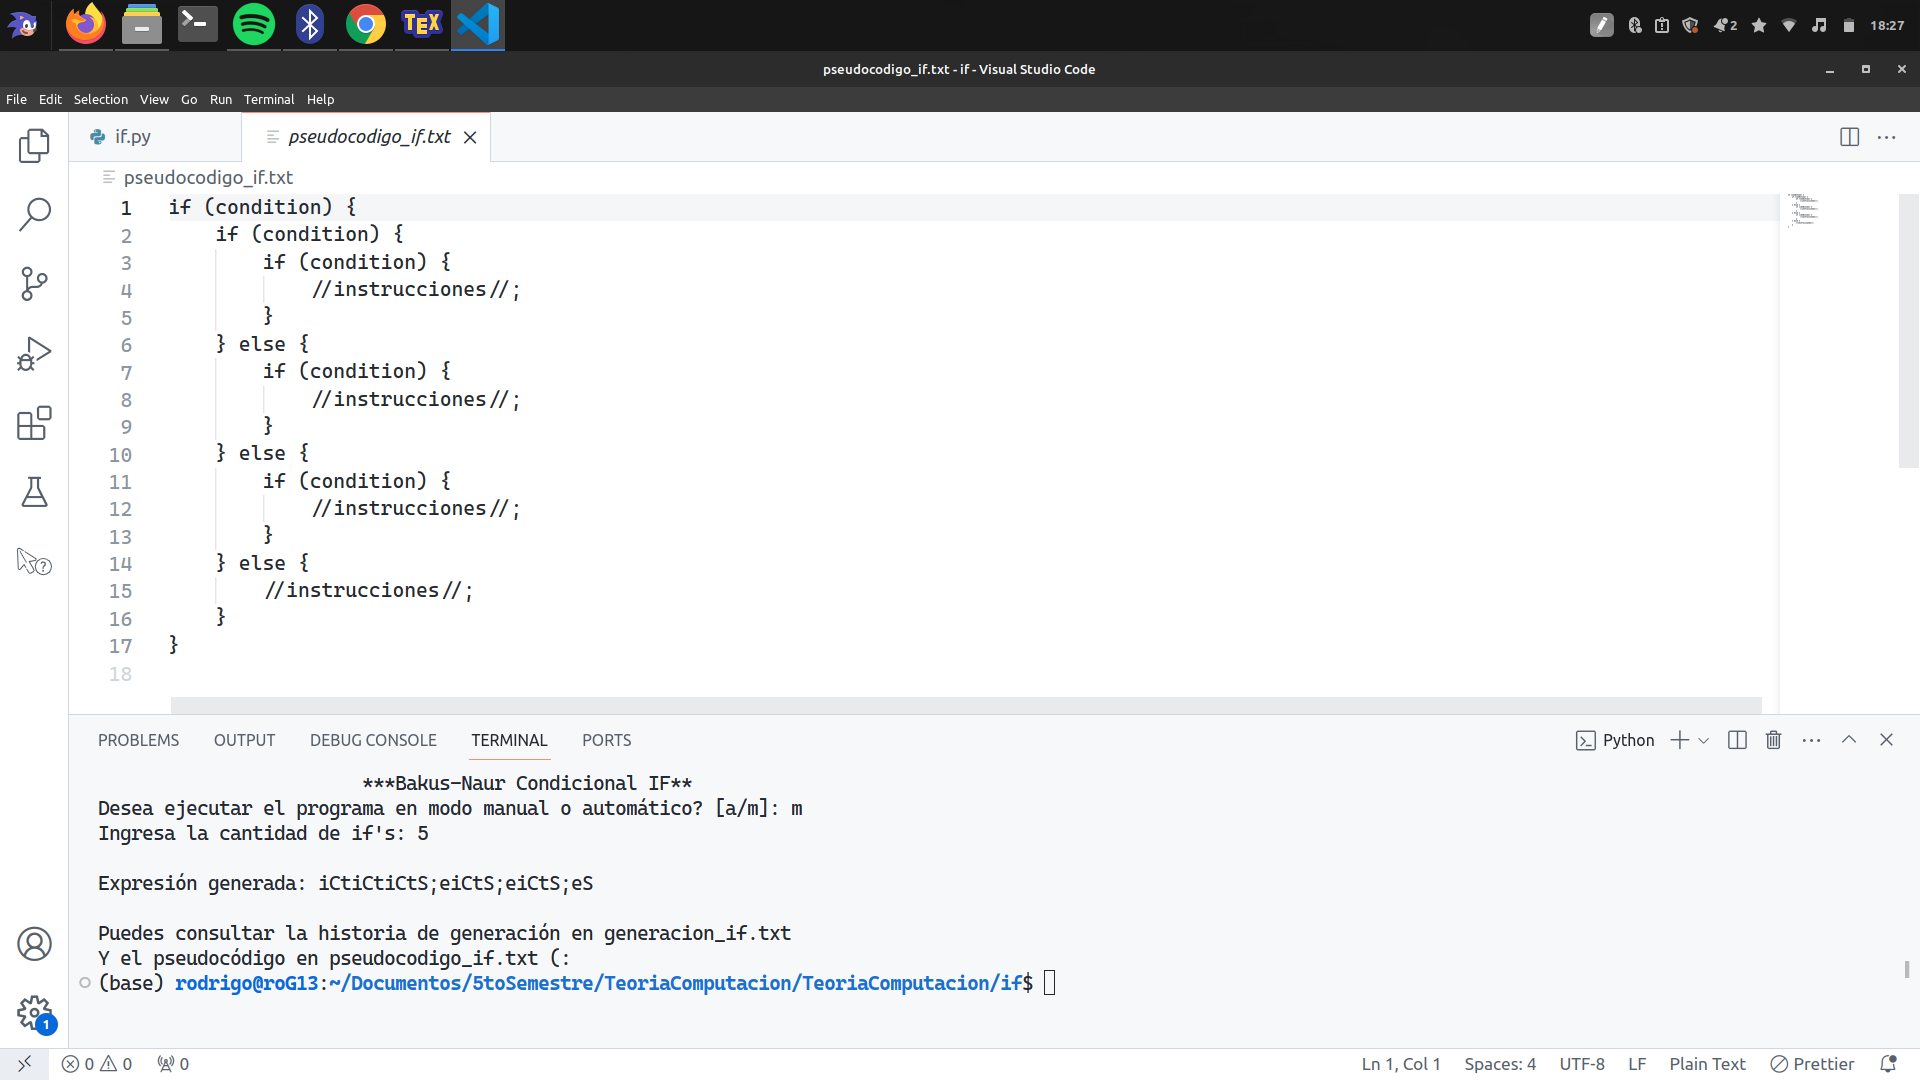
\includegraphics[width=0.8\textwidth]{3,2}
		\caption{Pseudocódigo del Modo manual 3 - Longitud 5}
	\end{figure}
	
	
	
	\newpage
	\begin{figure}[h]
		\centering
		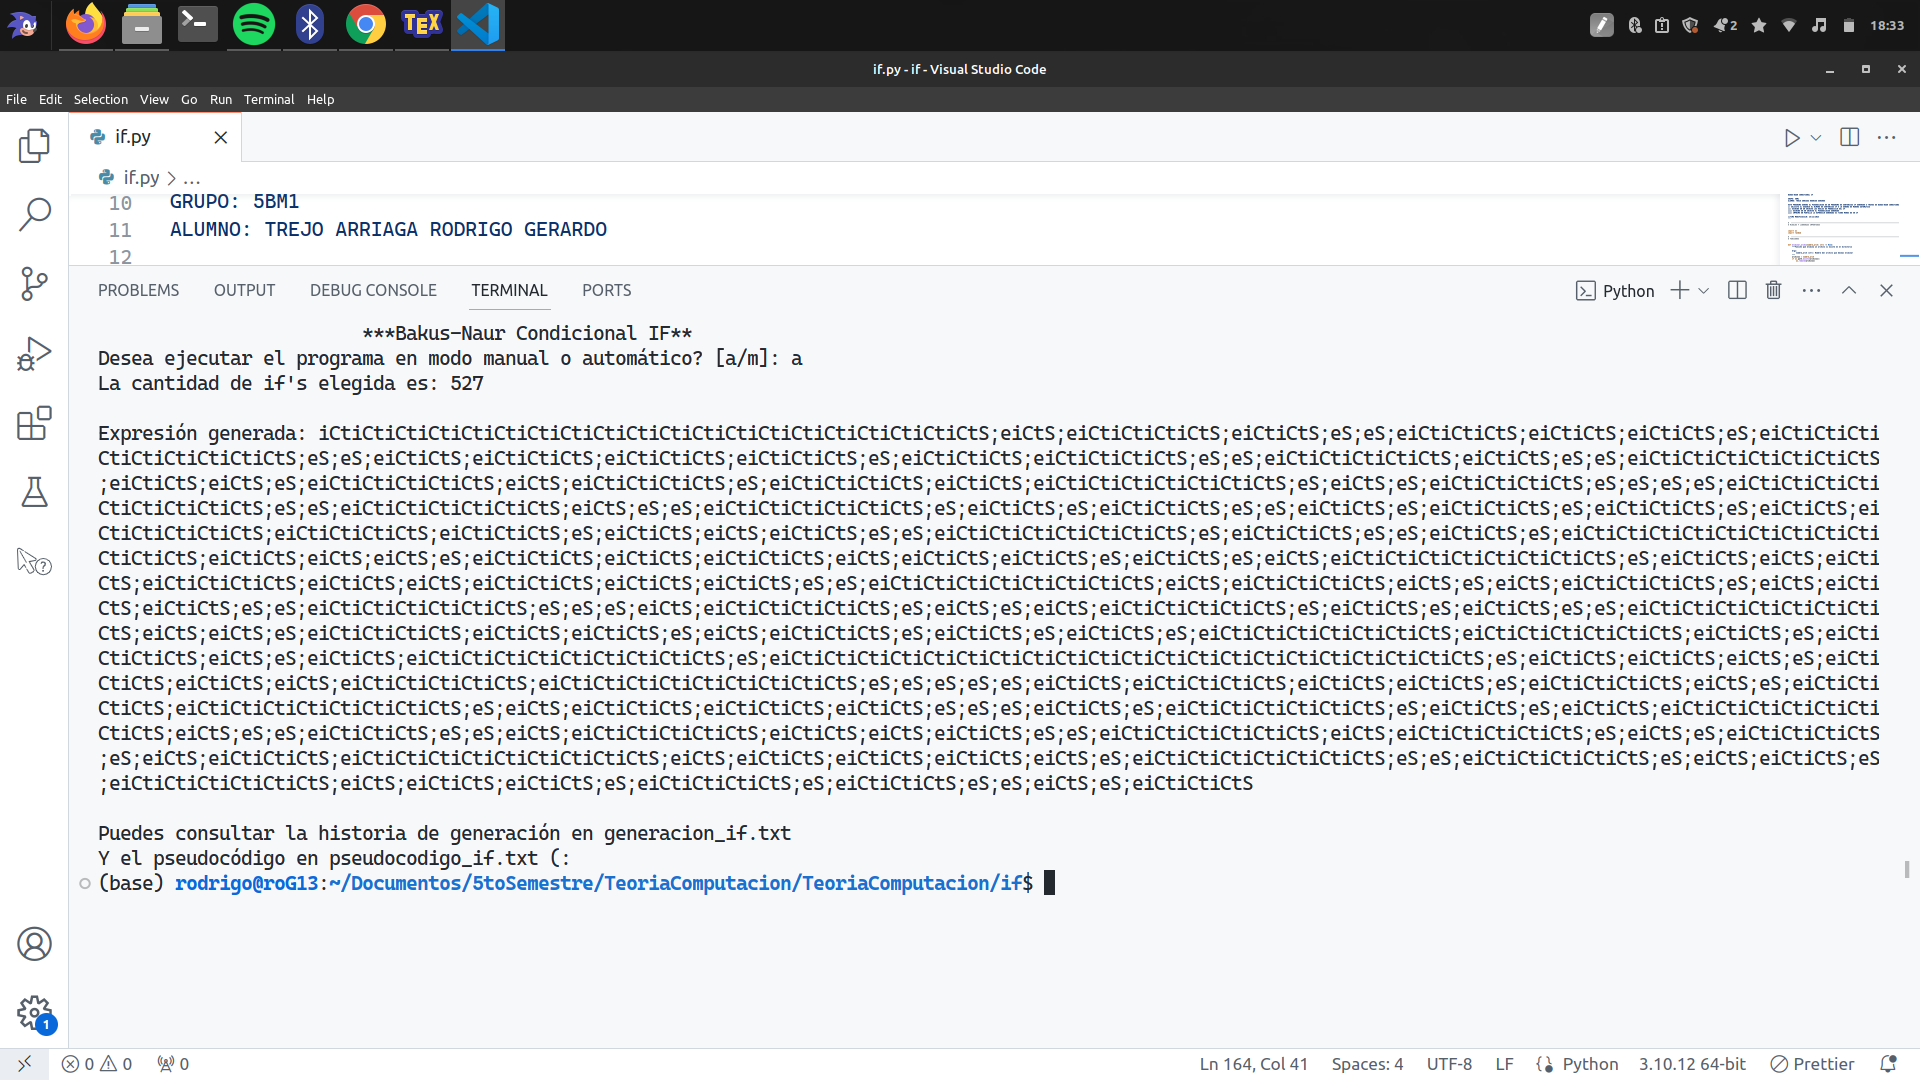
\includegraphics[width=0.8\textwidth]{auto.png}
		\caption{Modo automático}
	\end{figure}
	
	\begin{figure}[h]
		\centering
		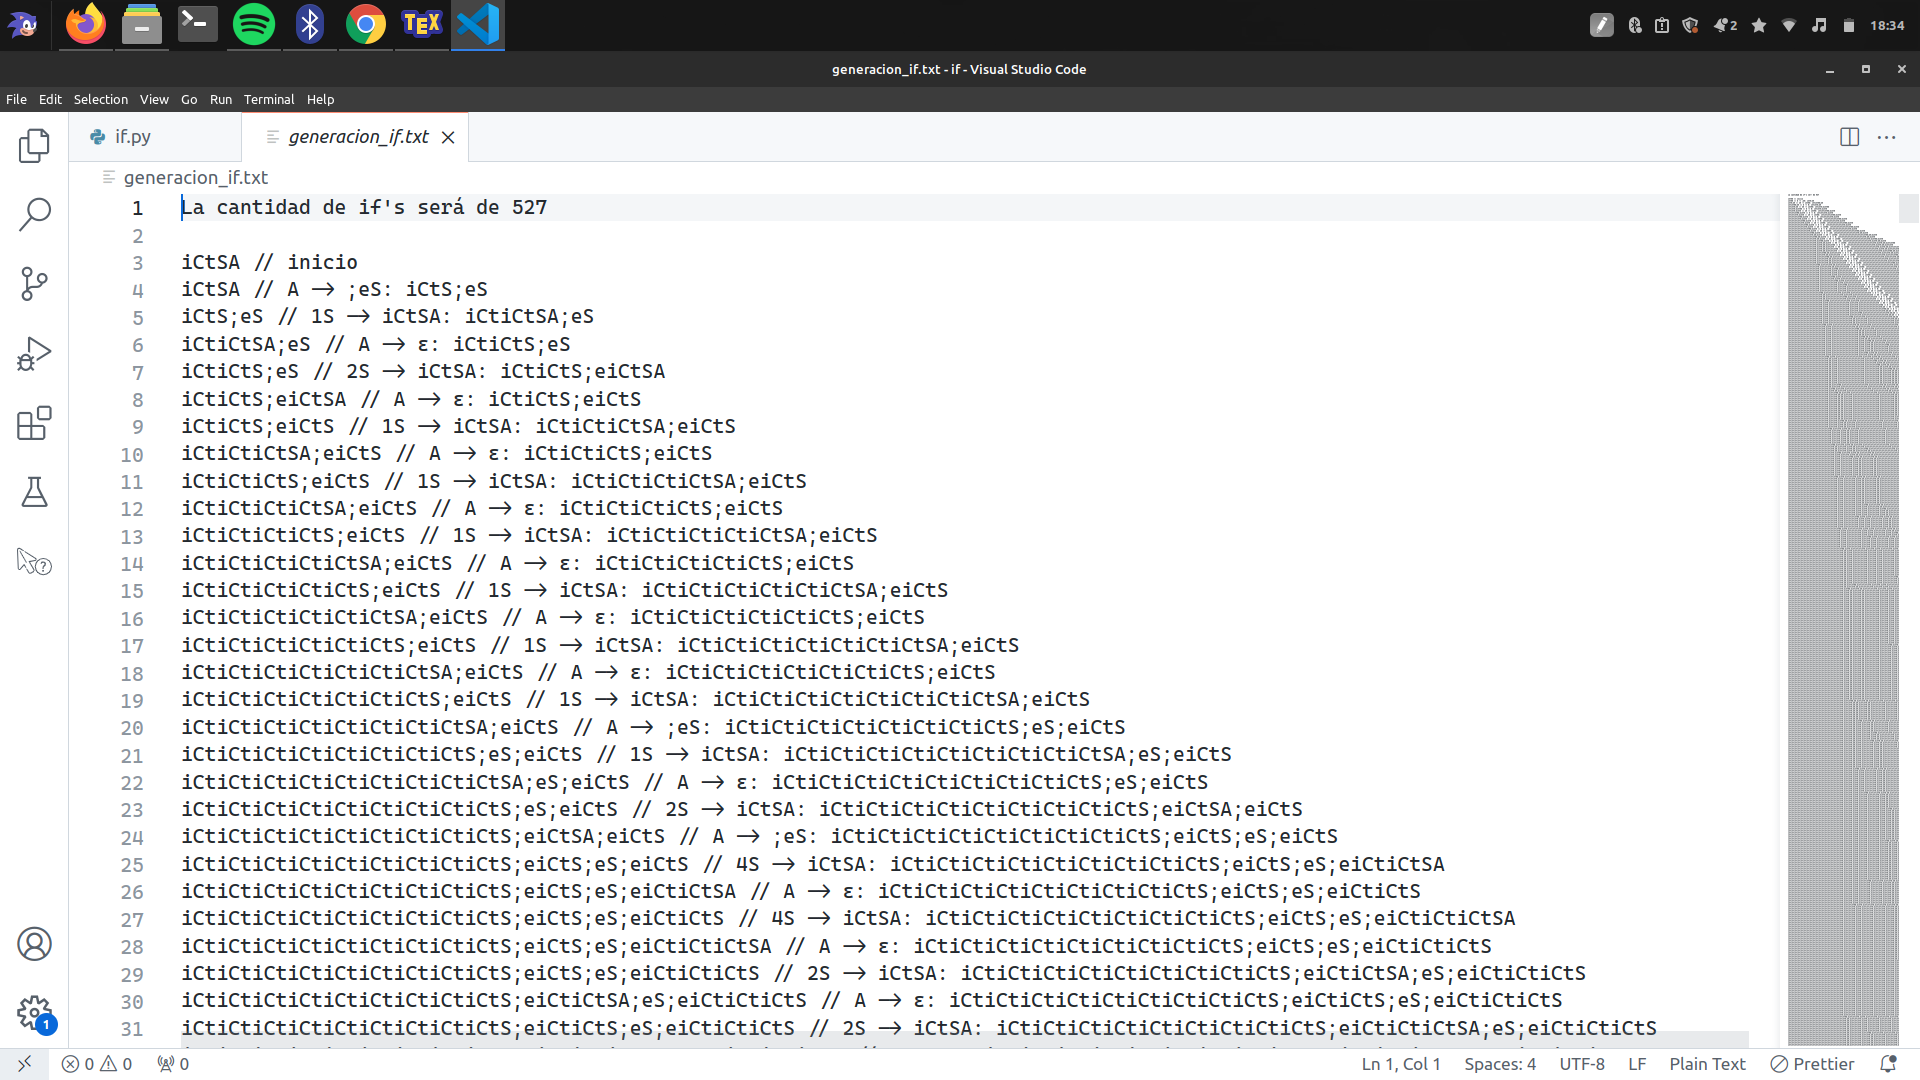
\includegraphics[width=0.8\textwidth]{arch4,1}
		\caption{Generación del Modo automático}
	\end{figure}
	
	
	\newpage
	
	\begin{figure}[h]
		\centering
		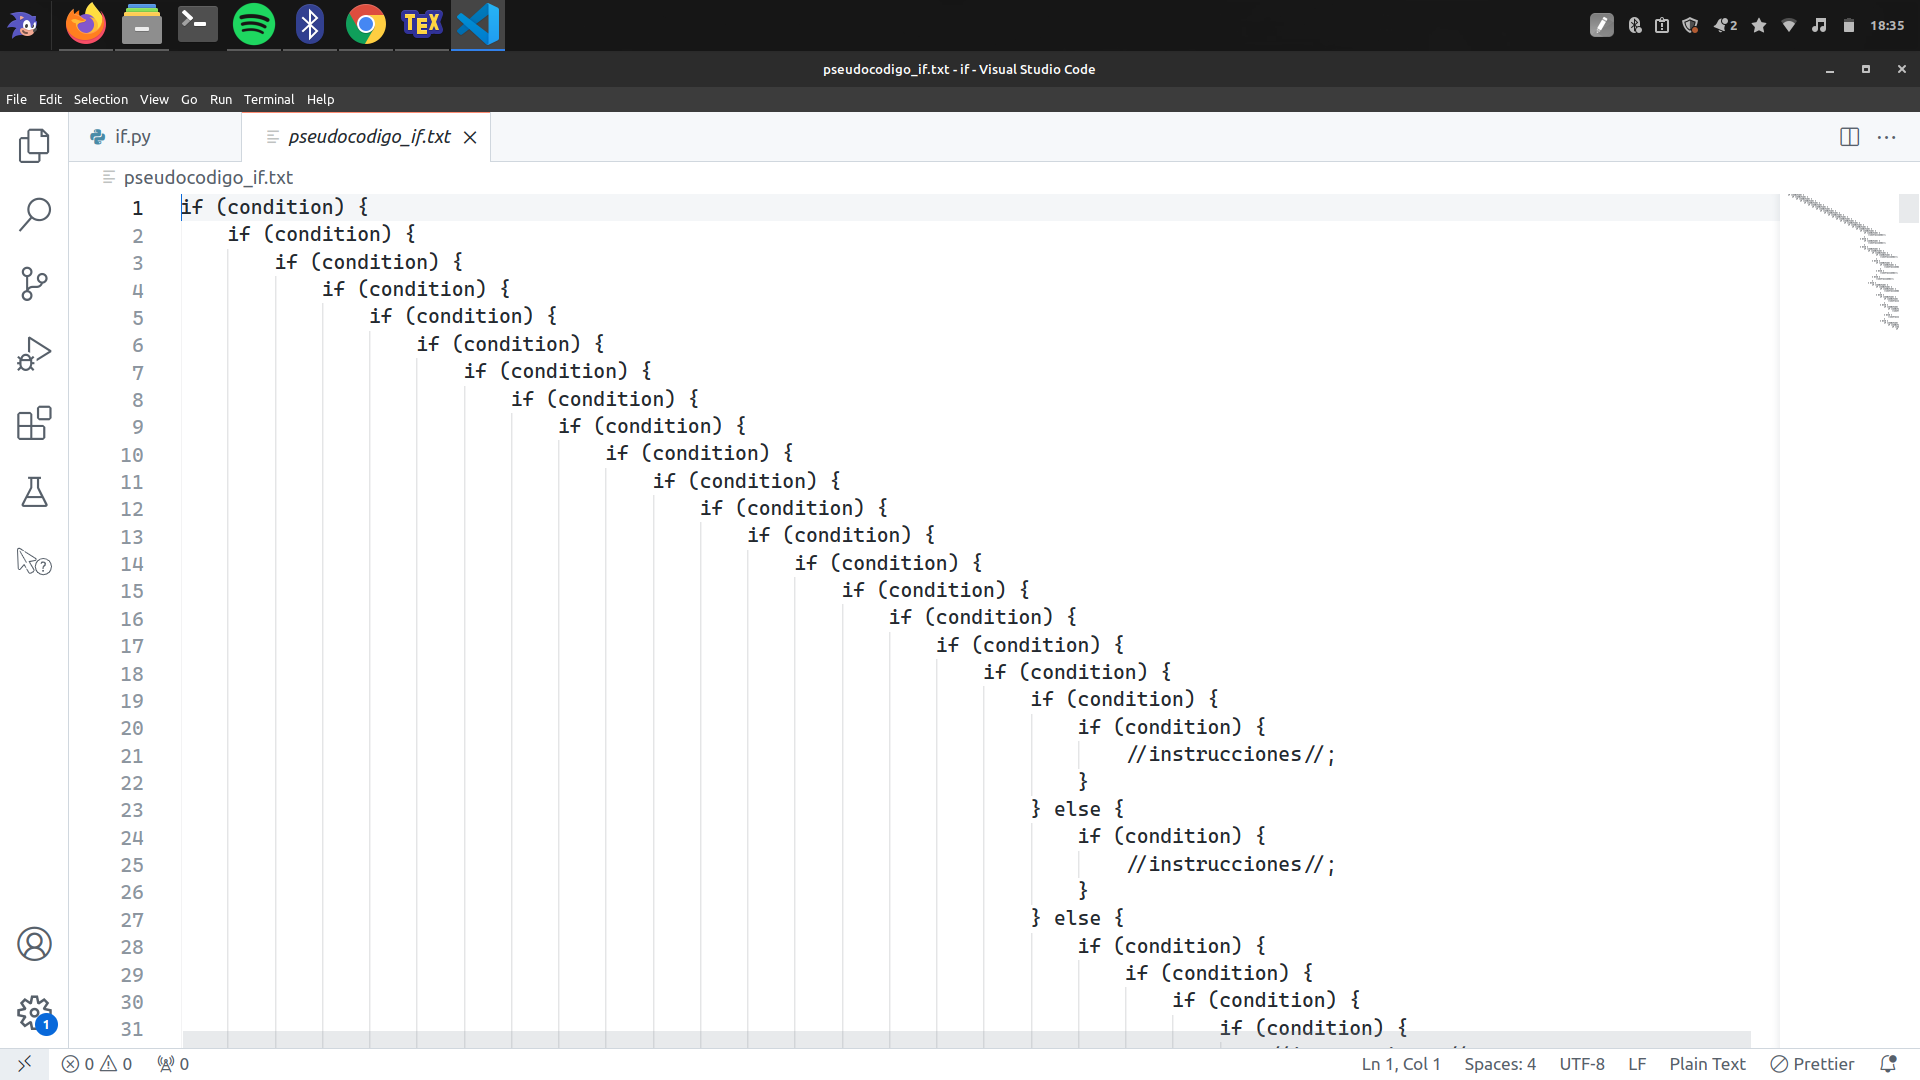
\includegraphics[width=0.8\textwidth]{arch4,2}
		\caption{Pseudocódigo del Modo automático}
	\end{figure}
	
	\section*{Conclusión}
	El desarrollo del programa para derivar la gramática de Backus-Naur del condicional IF ha sido una tarea complicada en principio pero sumamente instructiva. A través de la implementación de este programa, se ha demostrado la capacidad de las gramáticas libres de contexto para describir estructuras sintácticas complejas y la eficiencia de la notación BNF para representar estas gramáticas de manera concisa y precisa. 
	
	El ejercicio de derivar automáticamente una gramática hasta un número dado de estructuras condicionales ha reforzado la comprensión de los mecanismos de generación y análisis sintáctico que subyacen a los compiladores y a los intérpretes de lenguajes de programación. Además, la limitación de las derivaciones a un máximo de 1000 ha puesto de relieve la importancia de establecer restricciones prácticas para evitar la generación excesiva y la posibilidad de caer en bucles infinitos. 
	
	Esta práctica ha proporcionado una visión valiosa sobre la teoría de la computación y ha subrayado la relevancia de las estructuras de control, como la condicional IF, en la construcción de programas y en el flujo lógico de la ejecución. Las habilidades y conocimientos adquiridos durante esta práctica serán de gran utilidad para el análisis y diseño de lenguajes de programación en el futuro.
	
	
	
	\section*{Bibliografía}
	
	
	[1] AcademiaLab. “Gramática libre de contexto \_ AcademiaLab”. Home | AcademiaLab. Accedido el 24 de diciembre de 2023. [En línea]. Disponible: https://academia-lab.com/enciclopedia/gramatica-libre-de-contexto/
	
	[2] AcademiaLab. “Forma de Backus-Naur”. AcademiaLab. Accedido el 24 de diciembre de 2023. [En línea]. Disponible: https://academia-lab.com/enciclopedia/forma-de-backus-naur/
	
	[3] W. David. “Backus-Naur form (BNF)”. David A. Wheeler's Personal Home Page. Accedido el 24 de diciembre de 2023. [En línea]. Disponible: https://dwheeler.com/lovelace/bnf.htm
	
	
	
	\newpage
	\section{Anexo - Código de Implementación}
	
	\begin{lstlisting}
		
	'''
	INSTITUTO POLITECNICO NACIONAL
	ESCUELA SUPERIOR DE COMPUTO
	
	INGENIERIA EN INTELIGENCIA ARTIFICIAL
	
	TEORIA DE LA COMPUTACION
	BAKUS-NAUR CONDITIONAL IF
	
	GRUPO: 5BM1
	ALUMNO: TREJO ARRIAGA RODRIGO GERARDO
	
	ESTE PROGRAMA GENERA EL PSEUDOCODIGO DE UN PROGRAMA DE SENTENCIAS IF GENERADO A TRAVES DE BAKUS-NAUR CONDITIONAL IF:
	i) SOLICITA AL USUARIO EL NUMERO DE IF's O LO GENERA DE MANERA AUTOMATICA
	ii) ESCRIBE EN UN ARCHIVO LAS REGLAS DE PRODUCCION DEL IF
	iii) ESCRIBE EN UN ARCHIVO EL PSEUDOCODIGO GENERADO
	iii) IMPRIME EN PANTALLA LA EXPRESION GENERADA SI TIENE MENOS DE 50 IF
	
	ULTIMA MODIFICACION: 24/12/2023
	'''
	
	#  --------------------------------------------------------------------------------------------------------------------
	# MODULOS Y LIBRERIAS IMPORTADAS
	
	
	import os
	import random
	
	#  --------------------------------------------------------------------------------------------------------------------
	# FUNCIONES
	
	
	def eliminar_archs(nombre_arch: str) -> None:
		"""Funcion que elimina un archivo si existe en el directorio
		
		Args:
		nombre_arch (str): Nombre del archivo que deseas eliminar
		"""
		archivo1 = nombre_arch
		if os.path.exists(archivo1):
		os.remove(archivo1)
	
	
	def reemplazar_nesima_ocurrencia(cadena: str, c_reemplazar: str, c_reemplazo: str, n:int) -> str:
		"""
		Reemplaza la n-esima ocurrencia de un caracter en una cadena.
		
		Args:
		cadena (str): Cadena en la que se realizara el reemplazo.
		c_reemplazar (str): Caracter que se buscara y reemplazara.
		c_reemplazo (str): Caracter con el que se reemplazara la n-esima ocurrencia.
		n (int): Numero de ocurrencia que se desea reemplazar.
		
		Returns:
		str: Cadena resultante despues del reemplazo.
		"""
		contador = 0
		resultado = ""
		
		for char in cadena:
		if char == c_reemplazar:
		contador += 1
		if contador == n:
		resultado += c_reemplazo
		else:
		resultado += char
		else:
		resultado += char
		
		return resultado
	
	
	def format_bnf_to_pseudocode(expresion:str):
		"""
		Convierte una expresion en formato BNF (Backus-Naur Form) a pseudocodigo
		con estructuras de control if.
		
		Args:
		expresion (str): Expresion en formato BNF.
		
		Returns:
		str: Pseudocodigo resultante.
		"""
		nivel_ident = 0
		pseudocodigo = ""
		i = 0
		
		while i < len(expresion):
		if expresion[i] == 'i':
		pseudocodigo += ' ' * nivel_ident + 'if (condition) {\n'
			nivel_ident += 4 
			elif expresion[i] == 'e':
			nivel_ident -= 4
			pseudocodigo += ' ' * nivel_ident + '} else {\n'
			nivel_ident += 4
			elif expresion[i] == 'S':
			pseudocodigo += ' ' * nivel_ident + '//instrucciones//;\n'
			elif expresion[i] == ';':
			nivel_ident -= 4
			pseudocodigo += ' ' * nivel_ident + '}\n'
		
		i += 1
		
		while nivel_ident > 0:
		nivel_ident -= 4
		pseudocodigo += ' ' * nivel_ident + '}\n'
		
		return pseudocodigo
		
		
		def aplicar_bnif(expresion:str, num_ifs:int, arch_cadena, arch_pseudo) -> str:
		"""
		Aplica las reglas de produccion de una gramatica BNF condicional if para
		generar una expresion y su pseudocodigo asociado.
		
		Args:
		expresion (str): Expresion inicial en formato BNF.
		num_ifs (int): Numero de instrucciones if a generar.
		arch_cadena: Archivo para registrar la cadena generada.
		arch_pseudo: Archivo para registrar el pseudocodigo.
		
		Returns:
		str: Expresion resultante.
		"""
		print(f"La cantidad de if's elegida es: {num_ifs}") if op == "a" else None
		
		arch_cadena.write(f"La cantidad de if's sera de {num_ifs}\n\n")
		
		arch_cadena.write(f"{expresion} // inicio\n")
		
		while expresion.count("i") < num_ifs:
		if "A" in expresion:
		rand = random.choice(a_rules)
		arch_cadena.write(f"{expresion} // A -> {'e' if rand == '' else rand}: {expresion.replace('A', rand)}\n")
		expresion = expresion.replace("A", rand)
		
		else:
		rand = random.randint(1, expresion.count("S"))
		arch_cadena.write(f"{expresion} // {rand}S -> {s_rule}: {reemplazar_nesima_ocurrencia(expresion, 'S', s_rule, rand)  }\n")
		expresion = reemplazar_nesima_ocurrencia(expresion, "S", s_rule, rand)      
		arch_cadena.close()
		
		expresion = expresion.replace("A", "")
		
		pseudocode = format_bnf_to_pseudocode(expresion)
		
		arch_pseudo.write(pseudocode)
		arch_pseudo.close()
		return expresion
	
	
	#  --------------------------------------------------------------------------------------------------------------------
	# FUNCION PPRINCIPAL
	
	
	if __name__ == "__main__":
	
		conta_ifs = 1
		expresion = "iCtSA"
		a_rules = [";eS", ""]
		s_rule = "iCtSA"
		
		os.system('clear')
		nombre_arch_cadena = "generacion_if"
		eliminar_archs(f"{nombre_arch_cadena}.txt")
		arch_cadena = open(f"{nombre_arch_cadena}.txt", "a+", encoding="utf-8")
		
		nombre_arch_pseudo = "pseudocodigo_if"
		eliminar_archs(f"{nombre_arch_pseudo}.txt")
		arch_pseudo = open(f"{nombre_arch_pseudo}.txt", "a+", encoding="utf-8")
		
		print("\t\t\t***Bakus-Naur Condicional IF**")
		op = input("Desea ejecutar el programa en modo manual o automatico? [a/m]: ")
		while op!="a" and op != "m":
		print("Modo invalido, intentelo nuevamente ):")
		op = input("Desea ejecutar el programa en modo manual o automatico? [a/m]: ")
		
		num_ifs = int(input("Ingresa la cantidad de if's: ")) if op == "m" else random.randint(0, 1000)
		
		expresion = aplicar_bnif(expresion, num_ifs, arch_cadena, arch_pseudo)
		
		print(f"\nExpresion generada: {expresion}")
		print(f"\nPuedes consultar la historia de generacion en {nombre_arch_cadena}.txt")
		print(f"Y el pseudocodigo en {nombre_arch_pseudo}.txt (:")
		
		
	\end{lstlisting}
	
	
	
\end{document}